\chapter{Introduction}

Nowadays, computer systems have a central role in our society. Originally intended to be computing tools for mathematicians, their evolution made them a central component of our society. Thanks to the progress in technology and in engineering techniques, these systems are now used for a multitude of purposes in very different domains: from the medical field, to the avionics, without forgetting about the relatively novel \textsl{"Internet of Things"}.

The new domains in which these systems are used, required a redefinition of the concept of \textsl{"computer systems"}. Many of these systems must respect hard deadlines to fullfill their tasks, or there may be serious consequences which could result even in fatalities.

Whenever the system must respect hard deadlines, we refer to them as \textsl{Critical Systems}. If a failure of such systems may be catastrophic, with serious damages to the environment, the infrastructures, or human beings, we talk about \textsl{Safety Critical Systems}.

There are cases in which these systems perform in a physical environment. An example of such a system is an autonomous car: a system composed by a \textsl{computer system}, in charge of doing the computations needed to fulfill the assigned task, and a physical component, in charge of interacting with the environment by change both the states of it and of the system itself.

Because these systems are so pervasive and yet so dangerous, in case of a failure, to satisfy and guarantee their (usually) ultra-high \textsl{dependability} requirements is a key factor during the design and development phase.

The \textsl{dependability} of a System is a measure of how \textsl{"trustable"} a system is, i.e. its ability to provide a \textbf{correct service}.

A \textsl{failure} is an event that causes a disruption of the provided service.

\section{Dependability and Safety}

The \textsl{dependability} of a critical system is defined as an ensemble of \textsl{qualitative} and \textsl{quantitative} measures.
Some of the most important are listed here:

\begin{itemize}
	\item \textsl{Availability}: a function that measures the alternation between correct and incorrect service
	\vspace{0.4cm}
	\begin{itemize}
		\item[]
	$
		A(t)\: =\: \begin{cases}
		1\quad if\: a\ correct\: service\: is\: provided\: at\: time\: t \\
		0\quad otherwise
		\end{cases}
	$
	\vspace{0.2cm}
		\item[] $\mathbb{E}[A(t)]$, the expected value of the availibility, is the probability that the system is providing a correct service at time t
	\end{itemize}
\end{itemize}

\begin{itemize}
	\item \textsl{Reliability}: the ability of the system to provide a \textsl{continuous service}
	\vspace{0.4cm}
	\begin{itemize}
		\item[] $R(t)$: probability of providing a correct service in the interval $[0, t)$
	\end{itemize}
\end{itemize}

\begin{itemize}
	\item \textsl{Safety}: the absence of catastrophic consequences if a failure occurrs.
	\item The \textsl{Safety} of a system is more often defined as the \textsl{Mean Time to the next Catastrophic Failure}, because the safety requirements require a quantitative measure (e.g. one failure every $10^{n})$ years).
	\vspace{0.4cm}
	\begin{itemize}
		\item[] $S(t)$: probability that \textbf{no failure} occurrs in the interval $[0,t)$
		\vspace{0.2cm}
		\item[] $MTTF$: Mean time between the recovery from a failure and the next failure.
	\end{itemize}
\end{itemize}

\begin{itemize}
	\item \textsl{Maintenaibility}: the ability for easy maintenance and repair from a failure. This measure has an influence on the Availibility.
	\begin{itemize}
		\item[] $MTTR$: Mean Time to Repair the system from a failure
	\end{itemize}
\end{itemize}

\begin{itemize}
	\item \textsl{Coverage}: the measure of effectiveness of the system's fault-tolerance mechanisms, i.e. the ability of the system to prevent, avoid or correct failures
\end{itemize}

\newpage

A \textsl{threat} is a menace to the system's dependability, that is an \textsl{"event"} that makes the system provide an incorrect service. Threats may be of different kinds and come from many sources, such as wrong specification or a wrong implementation of a specification, accidents$\dots$
When considering the dependability of a system, we are interested in providing a \textsl{continuous correct service}. A \textsl{failure} is a transition from a state of \textsl{correct service} to a state of \textsl{incorrect service}.
When designing a Critical System, the need to reduce the possible transitions (failures) from these two sets, guides the development process.

\begin{figure}[h!]
	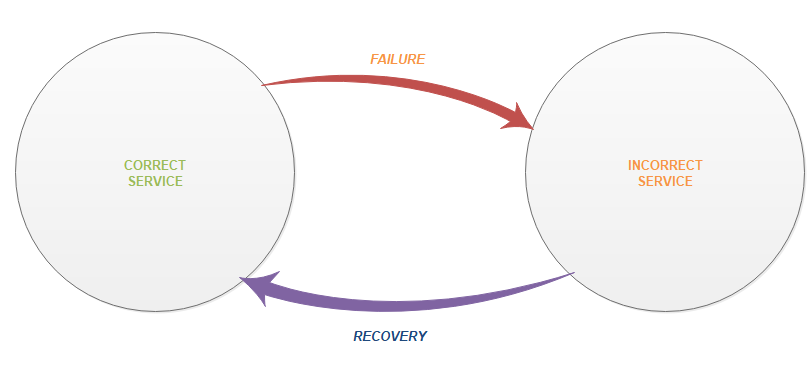
\includegraphics[width=\textwidth]{img/correct-incorrect.png}
	\caption{}
\end{figure}

When it comes to \textsl{Safety-Critical Systems}, we must distinguish between \textsl{benign failures} and \textsl{catastrophic failures}.
The first are failures that we can somehow accept: the system will not provid a correct service but it will still be in a safe state. The latter are the most dangerous kind of failures because an incorrect, unsafe service will potentially have catastrophic consequences such as damages to the environment, disruption of the system's infrastructure or even fatalities, in cases where these systems and humans work in close contact.
As an example, think to an autonomous car. Imagine that the car is riding in "normal" conditions and suddenly an obstacle appers in front of it. A screeching halt and a consequent interruption of the ride is indeed a failed state, but it's considered as a \textsl{benign safe}, because no one got hurt. On the other hand, a situation in which the car beging to throttle towards the obstacle and eventually collides with it, is defined as an \textsl{unsafe failure} because people in the car could get seriously injuried (or killed).
\newpage


\begin{figure}[h!]
	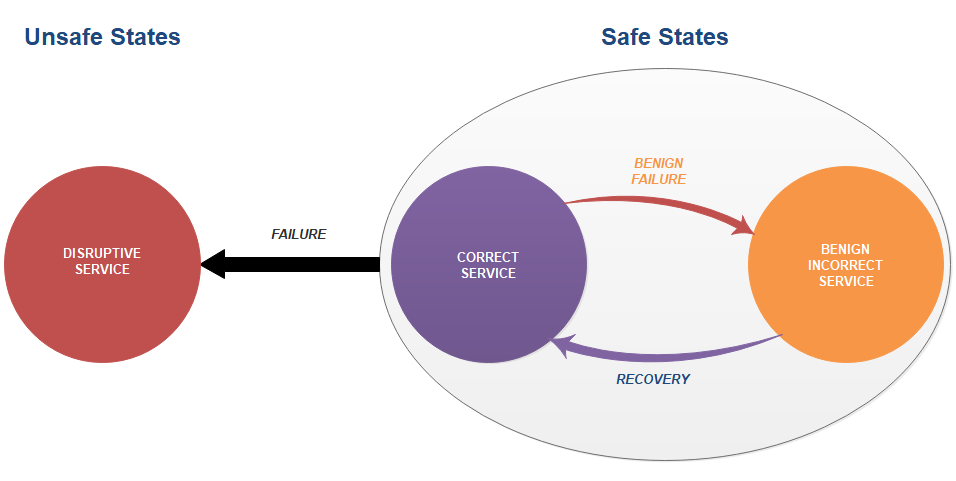
\includegraphics[width=\textwidth]{img/safe-unsafe.png}
	\caption{}
\end{figure}

To study the dependability of Safety-Critical Systems, we want to find all the possible failure causes. To do so, the academics agreed on the \textsl{fault-error-failure chain} model, which is widely accepted both by academics and practitioners:

\begin{itemize}
	\item \textsl{Fault}: the \textsl{adjudjed or hypothesized} cause of an error
	\item \textsl{Error}: that part of the system state that may cause a subsequent failure
	\item \textsl{Failure}: the situation in which the \textsl{error} reaches the service interface, altering the service of the whole system
\end{itemize}

\begin{figure}[h!]
	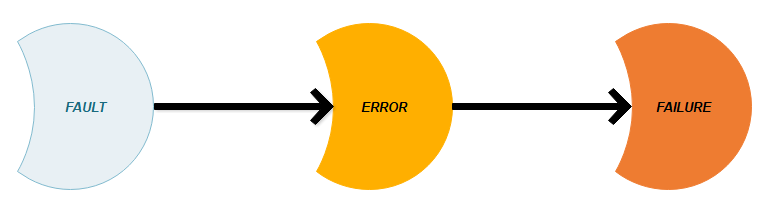
\includegraphics[width=\textwidth]{img/fault-error-failure.png}
	\caption{}
\end{figure}

The dependability of a system comes from a set of four techniques that aims to prevent/mitigate the consequences of possible failures:

\begin{itemize}
	\item \textsl{Fault Prevention}: means to prevent the occurence or introduction of failures
	\item \textsl{Fault Tolerance}: mechanisms to tolerate faults. In case of fault the system is still able to provide a correct service
	\item \textsl{Fault Removal}: reduction of the \textsl{number} or \textsl{severity} of faults in the system
	\item \textsl{Fault Forecasting}: use of statistical techniques to estimate the present number, the future incidence and the likely consequences of faults
\end{itemize}

The effectiveness of the measures adopted to achieve the dependability requirements of a system is measured through the \textsl{validation} process.
The validation of the system requirements is a process that must be repeated in each phase of the system development, even at the very beginning of the design phase.

There are multiple validation techniques that may be specifically selected for each phase of the system development:

\begin{itemize}
	\item \textsl{Analytical/Numerical Modeling}
	\begin{itemize}
		\item[-] Techniques that models the system capabilities using numerical models that have a closed form solution, i.e. the changes in a system can be described as mathematical analytic function. Examples of such models are the \textsl{Combinatorial} and the \textsl{State-Based} model
	\end{itemize}
	\item \textsl{Simulation}
	\begin{itemize}
		\item[-] Empirical estimation of the system dependability, deployed in a simulated environment. This method allows to inject faults, to check whether a specific fault-tolerance mechanism works or not		
	\end{itemize}
	\item \textsl{Measurement}
	\begin{itemize}
		\item[-] When a prototype of the system is available, its executions can be observed and the measures of interest computed
	\end{itemize}
\end{itemize}

It is important to keep in mind that these techniques are non-exclusive and the validation process should be a combination of these techniques. As said before, the process of validation should be done during the \textsl{whole} lifetime of a system, starting from the design phase and continuing after the deployment. Some of the methods listed above are more suitable than others in certain phases:

\begin{itemize}
	\item \textsl{Specification}: validation is done by the specification of the dependability requirements, that can be validated using Analytical/Numerical techniques, such as the \textsl{Combinatorial Models} to determine the failure conditions for the system's components. Failures are considered as independent
	\item \textsl{Design}: during the design phase, it's reasonable to model the state-space of the system using \textsl{State-Based Models}. Examples of such models are \textsl{Markov Chain}, \textsl{Petri Net} (and its evolutions)$\dots$
	\item \textsl{Implementation}: when the development is in an advance phase, it may be possible to build a prototype of the system that can be directly observed to measure the effectiveness of the fault-tolerance mechanisms on the system dependability
	\item \textsl{Operation}: once the system is deployed, it is possible to observe how it performs in a real environment
\end{itemize}

\section{System Monitoring}

The \textsl{Monitoring}

\section{Motivation and Goal of this work}